\documentclass[a4paper]{ctexart}
\usepackage{xeCJK}
\usepackage{setspace}
\usepackage{graphicx,wrapfig}
\usepackage{fontspec,xunicode,xltxtra}
\usepackage{fancyhdr,titlesec,titletoc}
\usepackage[titletoc]{appendix}
\usepackage[top=29mm,bottom=29mm,left=31.8mm,right=31.8mm]{geometry}
\usepackage{enumerate,enumitem}
\usepackage{caption,subcaption}
\usepackage{amsmath,amssymb,bm,array}
\usepackage{cite}
\usepackage{diagbox}
\usepackage{algorithm,algorithmicx,algpseudocode}
\usepackage{multirow}
\usepackage[super]{gbt7714}
\setmainfont{Times New Roman}
\setCJKmainfont[BoldFont={Songti SC Bold}]{SimSun}
\setCJKfamilyfont{heiti}{SimHei}
\renewcommand{\heiti}{\CJKfamily{heiti}\fontspec{Times New Roman}}
\renewcommand{\appendixpagename}{附录}

\usepackage{listings}
\usepackage[usenames,dvipsnames]{color}
\definecolor{MyDarkGreen}{rgb}{0.0,0.4,0.0}
\lstloadlanguages{Matlab}
\lstset{language=Matlab,
        frame=single,
        basicstyle=\small\ttfamily,
        keywordstyle=[1]\color{Blue}\bfseries,
        keywordstyle=[2]\color{Purple},
        keywordstyle=[3]\color{Blue}\underbar,
        identifierstyle=,
        commentstyle=\usefont{T1}{pcr}{m}{sl}\color{MyDarkGreen}\small,
        stringstyle=\color{Purple},
        showstringspaces=false,
        tabsize=5,
        morekeywords={xlim,ylim,var,alpha,factorial,poissrnd,normpdf,normcdf},
        morekeywords=[2]{on, off, interp},
        morekeywords=[3]{FindESS, homework_example},
        morecomment=[l][\color{Blue}]{...},
        numbers=left,
        firstnumber=1,
        numberstyle=\tiny\color{Blue},
        stepnumber=5
        }
\newcommand{\matlabscript}[2]
  {\begin{itemize}\item[]\lstinputlisting[caption=#2,label=#1]{#1.m}\end{itemize}}

\newcommand{\mycaptionfont}{\heiti\zihao{5}}
\captionsetup[figure]{name={\mycaptionfont 图},labelsep=period}
\captionsetup[table]{name={\mycaptionfont 表},labelsep=period}
\floatname{algorithm}{\mycaptionfont 算法}
\captionsetup[algorithm]{labelsep=period}
\renewcommand{\captionfont}{\mycaptionfont}
\renewcommand{\captionlabelfont}{\mycaptionfont}

\ctexset {
	section = {
		number = \arabic{section},
		format = \zihao{4}\bfseries,
	},
	subsection = {
		number = \arabic{section}.\arabic{subsection},
		format = \zihao{-4}\bfseries,
	},
	subsubsection = {
		number = \arabic{section}.\arabic{subsection}.\arabic{subsubsection},
		format = \zihao{-4}\bfseries,
	}
}
\setlist[enumerate]{itemindent=2em,listparindent=2em,leftmargin=0em,label=\arabic*、}

\setlength\parskip{.5\baselineskip}
\fancypagestyle{plain}{\pagestyle{fancy}}%改变章节首页页眉
\pagestyle{fancy}
\lhead{\kaishu~RFID无线射频识别实验报告~}
\rhead{\kaishu~1030616134~尹达恒}
\cfoot{\thepage}

\begin{document}

\begin{center}
	{\zihao{-3}\textbf{实验二\quad MATLAB编程实现ALOHA算法}}

	{\zihao{-4}尹达恒}\\[-1mm]

	{\zihao{5}(江南大学物联网工程学院,江苏\quad 无锡)}
\end{center}

\renewcommand{\baselinestretch}{1.3}
\zihao{-4}
\section{实验目的}
通过本次实验,进一步了解ALOHA算法,并将理论知识与实际相结合。

\section{实验设备}
MATLAB编程软件

\section{实验原理}\label{实验原理}
ALOHA法在多路存取方法中是最简单的,只要有一个数据包提供使用,这个数据包就被立即发送给射频读写器。ALOHA法是射频电子标签控制的,它只适用于只读射频电子标签。通常,这类射频电子标签只有一些数据传输给射频读写器,并且是在一个周期循环中将这些数据发送给射频读写器。数据传输时间只是循环周期的一小部分,所以在传输之间产生相当大的间隙;同时,各个射频电子标签的循环周期的差别可以忽略不计,各个射频电子标签的重复时间之间的差别是微不足道的。所以存在着一定的概率,两个射频电子标签可以在不同的时间段传输数据,使数据包不相互碰撞。
将时间分为离散的小段, 每一段称为时隙,每个时隙都足够让一个标签发送完信息; $N$个时隙合为一帧($N$是一个默认值) ;发射端随机选择一帧中的一个时隙向接收端发送信息,一旦发生碰撞,就在下一帧中随机选择一个时隙从新发送,如图\ref{fig:0}。
\begin{figure}[htbp]
	\centering
	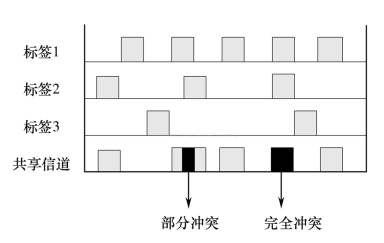
\includegraphics[width=0.6\textwidth]{figure/0.png}
	\caption{ALOHA算法碰撞图}\label{fig:0}
\end{figure}
平均交换的数据包量$G$可以用最简单的方法从一个数据包的传输持续时间$\tau$计算出来:

$$G=\sum_{1}^{n}\frac{\tau_n}{T}r_n$$

其中:$n$是系统中的标签数量,$r_n$为观察时间$T$内由应答器发送的数据包的数量。
传输信道的平均吞吐率$S$可由交换的数据包量G得出:
$$S=Ge^{-2G}$$
可以得出当$G=0.5$时, 最大吞吐率$S=1/(2e)=18.4\%$。

\section{实验步骤}
编写ALOHA模拟算法,依据第\ref{实验原理}节所介绍的ALOHA算法原理,可以得到ALOHA模拟算法流程如算法\ref{alg}所示。

\begin{algorithm}
	\caption{ALOHA模拟算法流程}
	\label{alg}
	\begin{algorithmic}[1]
		\Require 标签数量$m$
		\Require 各标签发送数据次数$n$
		\Require 各标签发送信息的时间$\bm B=\left\{b_{ij}\right\}$
		\Require 各标签的观察时间$\bm T$
		\Require 数据包宽度$T_0$
		\State 将$\bm B$各元素按大小排序以便于查找冲突
		\For{按时间顺序遍历$\bm B$中每个时间点$b_{ij}$}
		\If{$b_{ij}\le T$}
		\State 发送数据
		\If{$b_{ij}-min\left\{b|b\in\bm B\wedge b<b_{ij}\right\}\ge T_0$且$max\left\{b|b\in\bm B\wedge b>b_{ij}\right\}-b_{ij}\ge T_0$}
		\State 发送成功
		\Else 
		\State 发送失败
		\EndIf
		\EndIf
		\EndFor
		\Ensure 统计发送成功和发送失败的次数并绘图
	\end{algorithmic}
\end{algorithm}

按照算法\ref{alg}所示的算法流程编写matlab程序,运行结果如图\ref{fig:1}和\ref{fig:2}。

\begin{figure}[htbp]
	\centering
	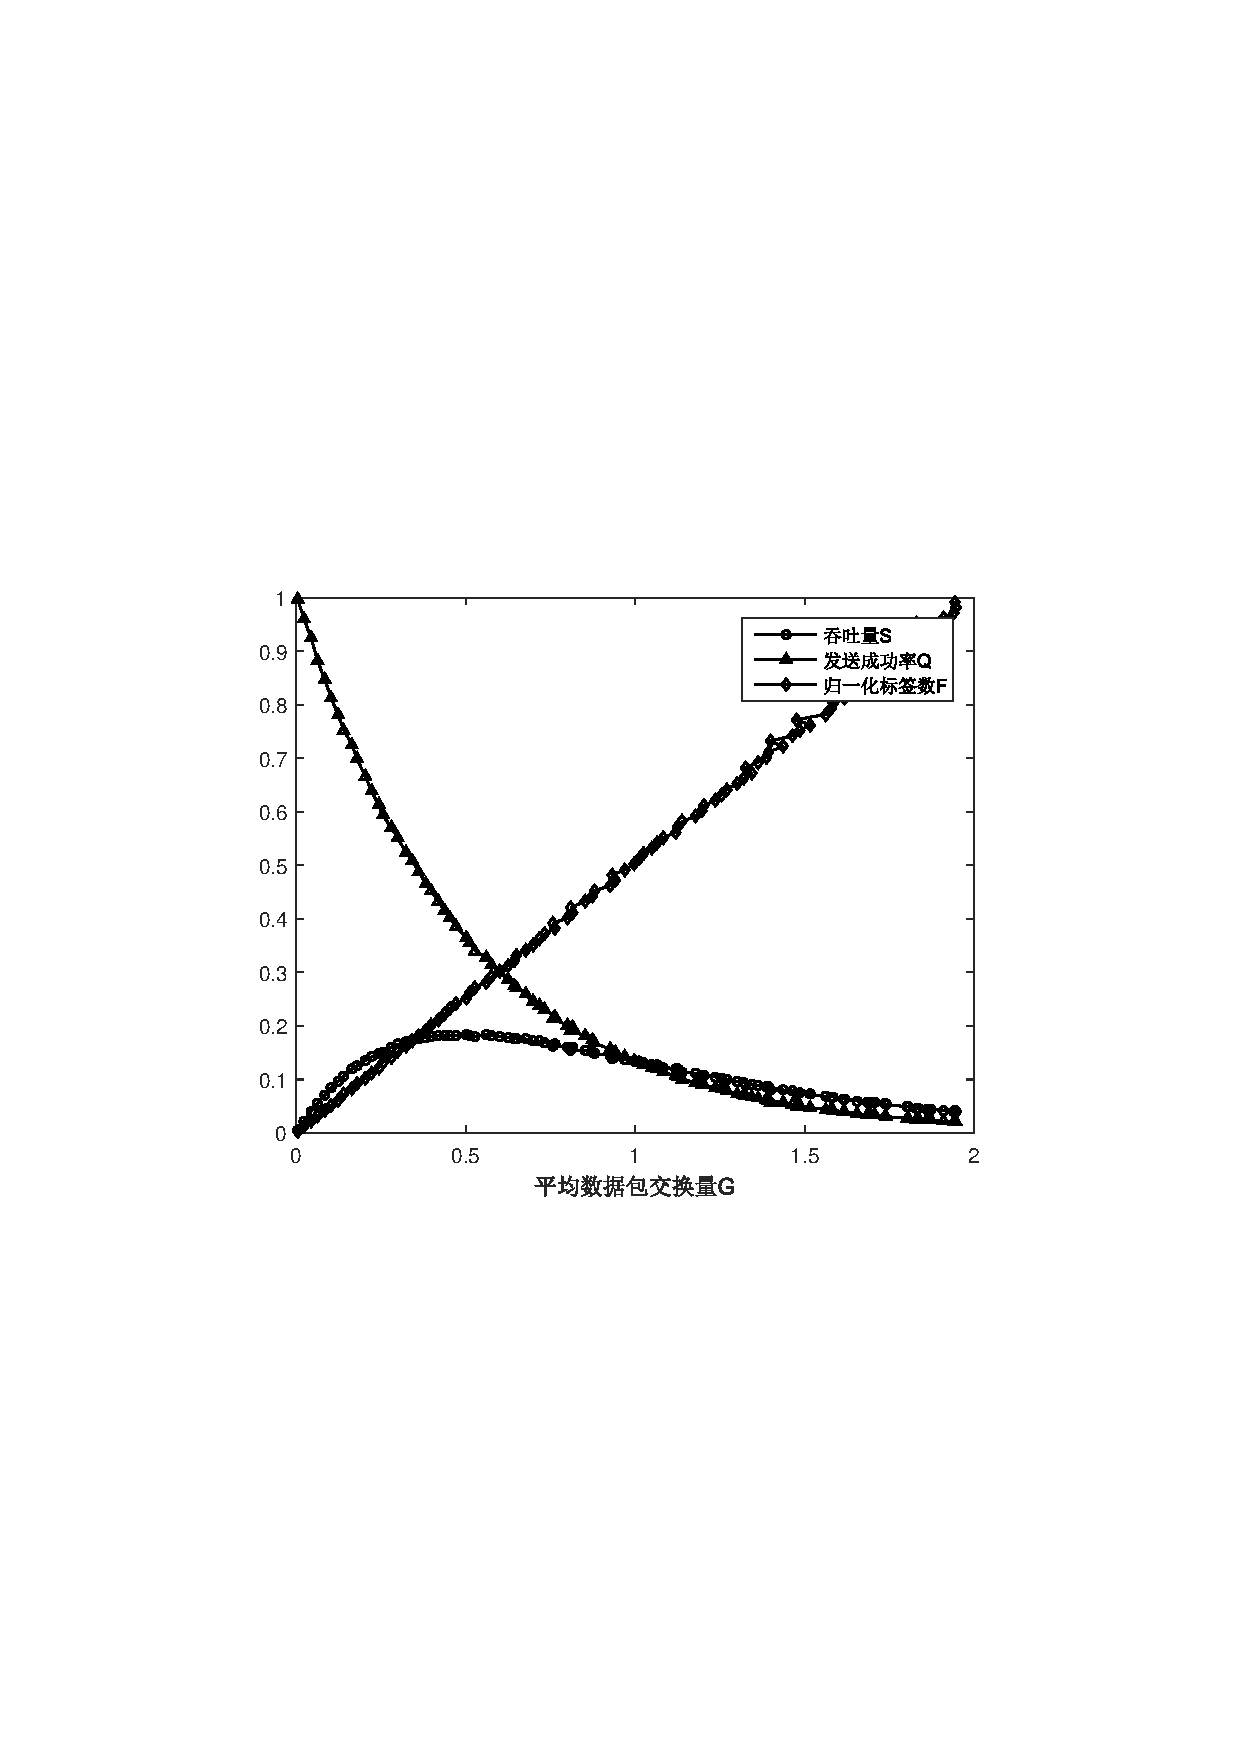
\includegraphics[width=0.8\textwidth]{figure/1.pdf}
	\caption{ALOHA算法模拟结果}\label{fig:1}
\end{figure}
\begin{figure}[htbp]
	\centering
	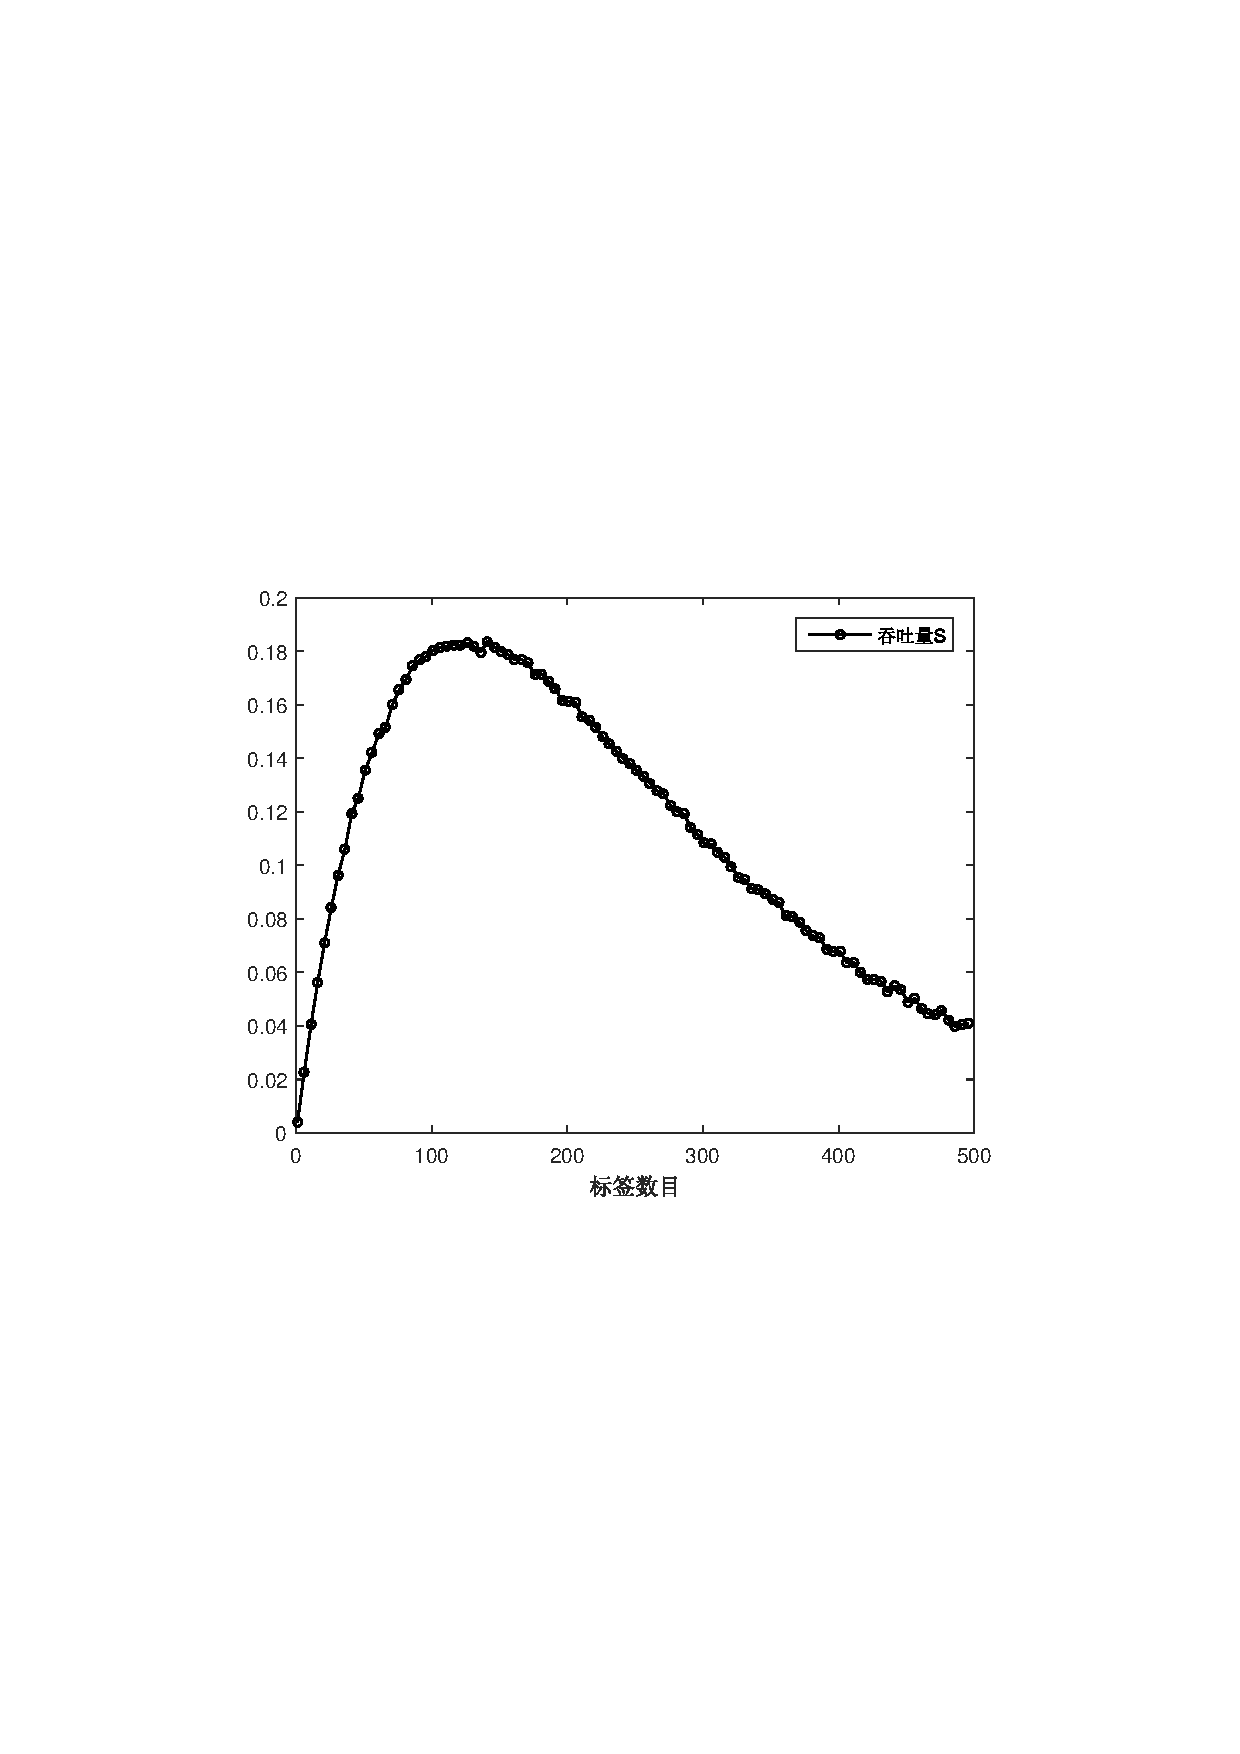
\includegraphics[width=0.8\textwidth]{figure/2.pdf}
	\caption{ALOHA算法模拟结果}\label{fig:2}
\end{figure}

\section{实验结果分析}
\begin{enumerate}
	\item 由图\ref{fig:1}可以看出随着数据包交换量的增大,ALOHA网络的数据吞吐量在数据包交换量较小时上升,数据包交换量到达一定值后又开始下降,这是由于在数据包交换量较小时网络可以成功发送所有的数据包,因此数据表越多网络吞吐量越大,而当数据包交换量达到一定值后,网络出现拥塞,要发送的数据包越多,互相之间的干扰也越大,发送成功率下降,从而网络的吞吐量下降;
	\item 由图\ref{fig:2}可以看出,随着标签数目的增大,ALOHA网络的数据吞吐量也呈先上升后下降的趋势,其原因类似,是由于标签量较少时不容易出现拥塞,而标签量较大时使网络出现拥塞所致。
\end{enumerate}

\newpage
\appendix
\appendixpage
\section{实验代码}
\begin{lstlisting}
Tag_num=500;
ym=1:5:Tag_num;
G=zeros(size(ym));
S=zeros(size(ym));
Q=zeros(size(ym));
F=zeros(size(ym));
k=1;
for m=ym
	n=1000;
	A=rand(m,n);
	A1=0.5*A;
	B=cumsum(A1,2);
	T=B(1,n);
	C=1:1:(m*n);
	for i=1:m
		for j=1:n
			C(1,(i-1)*n+j)=B(i,j);
		end
	end
	D=sort(C);
	E=diff(D);
	T0=0.001;
	N=0;
	M=0;
	for i=1:(m*n-1)
		if D(1,i)<=T
			M=M+1;
			if i==1&&E(1,1)>=T0
				N=N+1;
			elseif i==(m*n-1)&&E(1,(m*n-1))>=T0
				N=N+1;
			elseif i~=1&&i~=(m*n-1)&&E(1,i)>=T0&&E(1,i-1)>=T0
				N=N+1;
			end
		else continue
		end
	end
	G(k)=T0/T*M;
	S(k)=T0/T*N;
	Q(k)=S(k)/G(k);
	F(k)=m/Tag_num;
	k=k+1;
end
markersize=4;
figure(1)
plot(G,S,'k-o','linewidth',1,'markersize',markersize);
hold on
plot(G,Q,'k-^','linewidth',1,'markersize',markersize);
hold on
plot(G,F,'k-d','linewidth',1,'markersize',markersize);
hold on
xlabel('平均数据包交换量G');
legend('吞吐量S','发送成功率Q','归一化标签数F');
figure(2)
plot(ym,S,'k-o','linewidth',1,'markersize',markersize)
legend('吞吐量S')
xlabel('标签数目')
\end{lstlisting} 
\end{document}